\documentclass[12pt,a4paper]{article}
\renewcommand{\baselinestretch}{1.05}
\usepackage[spanish]{babel}
%\usepackage[utf8]{inputenc}

\usepackage{amsmath,amsthm,verbatim,amssymb,amsfonts,amscd, graphicx}
\usepackage{graphicx}
\usepackage{caption}
\usepackage{subcaption}
\usepackage{tkz-fct}
\usetikzlibrary{babel}
\usepackage{pgfplots}
\usepackage{booktabs}
\usepackage{float}
\usepackage{enumitem}
\usepackage{forest}
\usepackage{hyperref}

%Uso de la fuente Source Sans Pro

\usepackage[default]{sourcesanspro}
%\usepackage[T1]{fontenc}

%Controlar la partición de palabras.
\pretolerance=5000
\tolerance=6000

%Simbolo de euro
\usepackage{eurosym} % para el euro


%Definición de monospace para codigo inline y paquete listings para código fuente.
\def\code#1{\texttt{#1}}
\usepackage{listingsutf8}
\lstset{
    %extendedchars=false,
    %inputencoding=utf8
}
\usepackage{color}
\definecolor{grisclarito}{gray}{0.95}

\lstdefinestyle{customc}{
  %belowcaptionskip=1\baselineskip,
  breaklines=true,
  frame=single,
  %xleftmargin=\parindent,
  language=C,
  showstringspaces=false,
  %basicstyle=\ttfamily,
  keywordstyle=\bfseries\color{green!40!black},
  commentstyle=\itshape\color{purple!40!black},
  identifierstyle=\color{blue},
  stringstyle=\color{orange},
  backgroundcolor=\color{grisclarito}
}

\hypersetup{
  colorlinks=true,
  linkcolor=black,
  urlcolor=blue
}

\setlength{\parindent}{0pt}
\topmargin0.0cm
\headheight0.0cm
\headsep0.0cm
\oddsidemargin0.0cm
\textheight23.0cm
\textwidth16.5cm
\footskip1.0cm

\renewcommand*\contentsname{Índice}
\newcommand{\mylabel}[2]{#2\def\@currentlabel{#2}\label{#1}}

\begin{document}
\begin{titlepage}
  \centering
  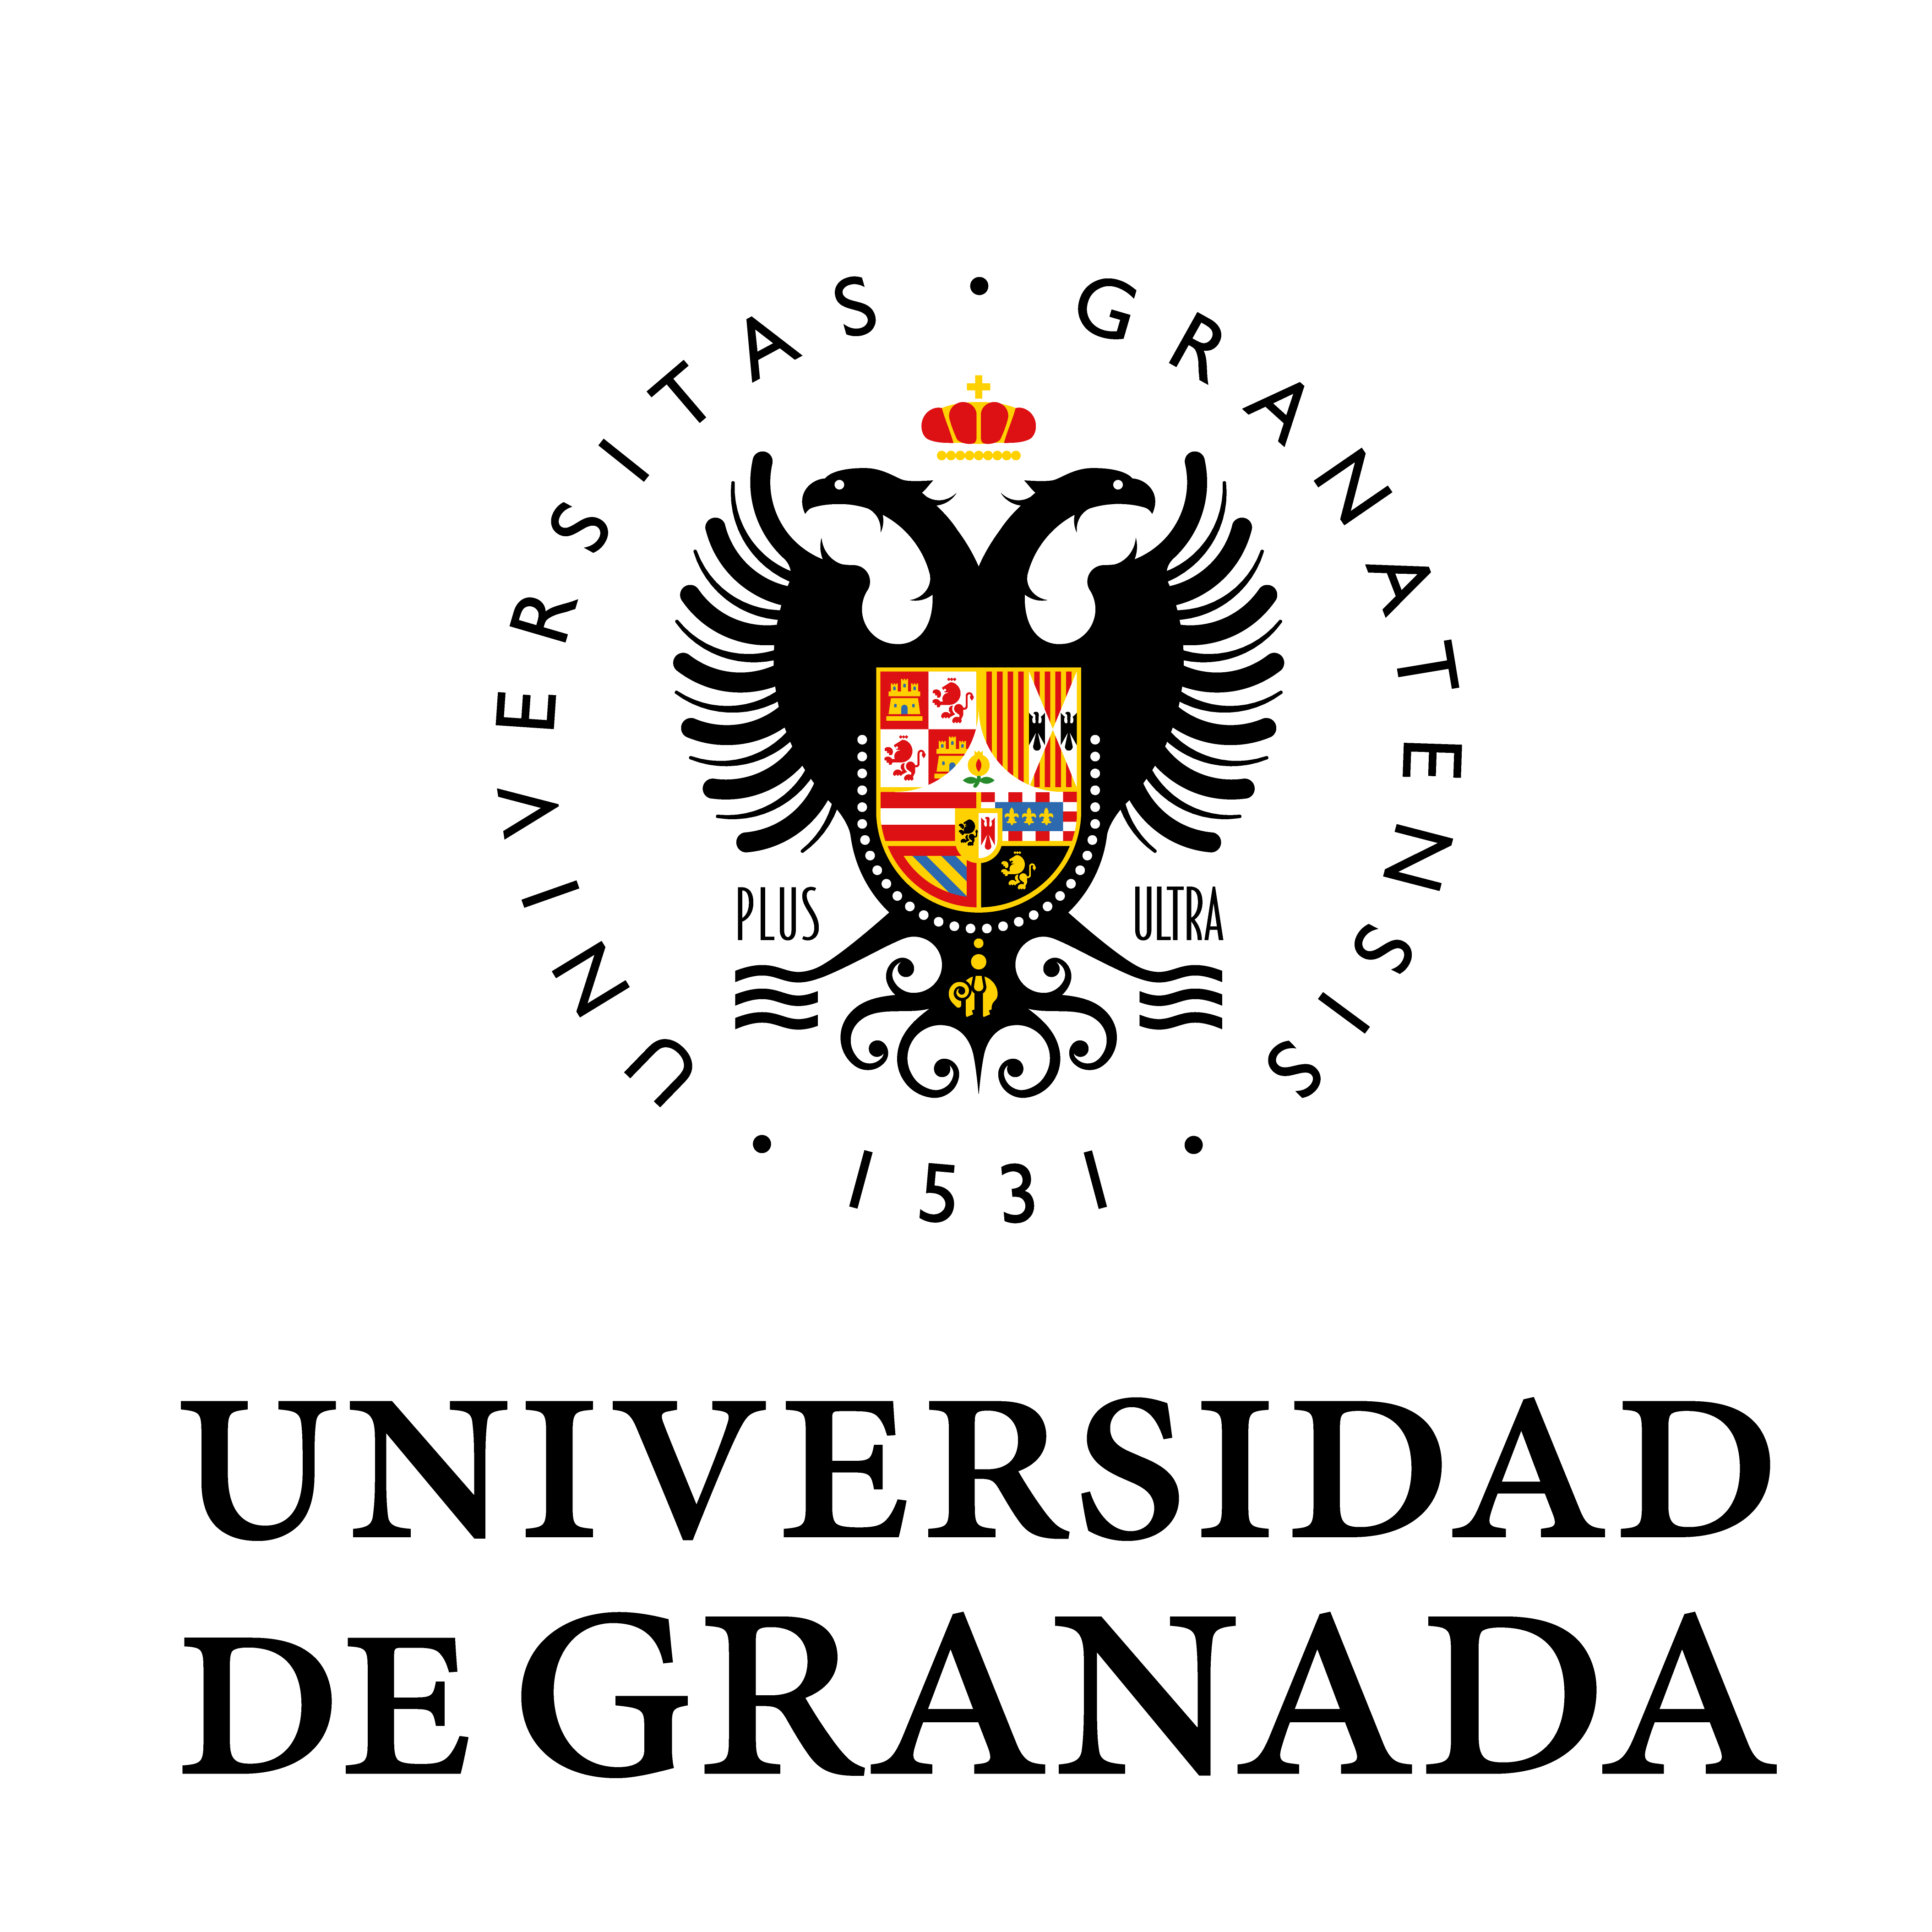
\includegraphics[width=0.6\textwidth]{imagenes/ugr.png}\par\vspace{1cm}
  {\scshape\large Diseño y Desarrollo de Sistemas de Información \par} \vspace{1cm}
  {\huge\bfseries Diseño de un sistema de información para la gestión y reproducción de música. \par}
  \vspace{0.4cm}
  {\large\itshape P1.Descripción del sistema y especificación de requisitos\\}
  \vspace{0.6cm}
  {\large\itshape  Darío Abad Tarifa \\ Juan Francisco Díaz Moreno \\ Pedro Domínguez López \\ Javier Sáez de la Coba \par} \vspace{1.00cm}
  Curso 2018-2019 \\
  \vfill

  % Bottom of the page
  {\large \today\par}
\end{titlepage}

\tableofcontents
\newpage

\setlength{\parskip}{10pt}

\section{Descripción del problema a resolver.}

Una empresa de streaming de audio quiere rehacer su plataforma de gestión de música (todo el servicio excepto el propio streaming de música). Para ello requiere que puedan haber cuentas de oyentes y de artistas.

El sistema ofrece diferentes opciones de carácter social para facilitar la relación entre amigos y los artistas con sus oyentes. Un usuario puede seguir a otro usuario (sea artista o no) para estar al corriente de lo que escucha proporcionando el nombre del usuario al que quiere seguir. Un usuario podrá recomendar una canción a otro usuario proporcionando el nombre de este y el identificador de la canción que quiere recomendar. Un usuario podrá solicitar un resumen sobre las canciones que escucha su lista de amigos. 
Un usuario podrá ver las recomendaciones que le llegan de sus amigos. Además, los usuarios oyentes pueden valorar las canciones que escuchan. Por último podrán visualizar las canciones mejor valoradas por un usuario proporcionando su nombre de usuario.

\section{Análisis de requisitos.}

\subsection{Requisitos de datos}

\begin{enumerate}[label=\textnormal{RD\arabic*.}]

	\item Identificador de la canción, álbum o lista para escuchar: \label{rd1}
		\begin{itemize}
			\item Elección (canción, álbum o lista)
			\item Identificador
		\end{itemize}
		
	\item Datos de álbum almacenado: \label{rd2}
		\begin{itemize}
			\item Nombre del álbum
			\item Nombre del artista
			\item Fecha de introducción
			\item Identificador del álbum
        	\item Nombre del álbum
		    \item Nombre del artista
		    \item Fecha de introducción
			\item Número de canciones
			\item Duración
		\end{itemize}
		
		
	\item Datos de canción almacenada: \label{rd3}
		\begin{itemize}
			\item Identificador de la canción
		    \item Nombre de la canción
		    \item Nombre del artista
		    \item Nombre del álbum
		    \item Estilo de la canción
		    \item Duración de la canción
		    \item Fecha de introducción
		    \item Archivo de audio
		    \item Número de reproducciones
		    \item Valoración media
		\end{itemize}
		
	\item Datos de lista almacenada: \label{rd4}
		\begin{itemize}
		    \item Identificador de la lista
		    \item Nombre de la lista
		    \item Canciones que contiene
		    \item Duración de la lista
		    \item Fecha de creacion
		    \item Usuario al que pertenece
		    \item Seguidores
		\end{itemize}
		
	\item Identificador de la nueva lista creada: \label{rd5}
		\begin{itemize}
			\item Identificador de la lista
		\end{itemize}
		
	\item Nombre para la busqueda de una cancion, album o lista: \label{rd6}
		\begin{itemize}
			\item Nombre
		\end{itemize}
		
	\item Lista con los posibles identificadores según el resultado de la búsqueda: \label{rd7}
		\begin{itemize}
			\item Identificador
			\item Tipo: canción, álbum, lista
			\item Nombre
			\item Usuario o artista
			\item Fecha de publicación o de creación
			\item Duracionr
		\end{itemize}
		
	\item Datos para crear una lista nueva: \label{rd8}
		\begin{itemize}
			\item Usuario
			\item Fecha 
		\end{itemize}
		
	\item Valoración de una canción: \label{rd9}
		\begin{itemize}
			\item Identificador de la canción
			\item Identificador
		\end{itemize}
		
	\item Datos nuevo álbum: \label{rd10}
		\begin{itemize}
		    \item Nombre del álbum
		    \item Nombre del artista
		    \item Fecha de introducción
		\end{itemize}
		
	\item Datos nueva canción: \label{rd11}
		\begin{itemize}
		    \item Nombre de la canción
		    \item Nombre del artista
		    \item Nombre del álbum
		    \item Estilo de la canción
		    \item Duración de la canción
		    \item Fecha de introducción
		    \item Archivo de audio
		\end{itemize}
		
	\item  Identificador de la canción introducida: \label{rd12}
		\begin{itemize}
			\item Identificador de la canción
		\end{itemize}
		
	\item Identificador de la canción para ver sus estadísticas: \label{rd13}
		\begin{itemize}
			\item Identificador de la canción
		\end{itemize}
		
	\item Reproduccion de una lista: \label{rd14}
		\begin{itemize}
		   	\item Audio de las canciones de la lista
		\end{itemize}
		
	\item Estadísticas de la canción: \label{rd15}
		\begin{itemize}
		    \item Nombre de la canción
		    \item Número de reproducciones
		    \item Valoración media
		\end{itemize}
		
	\item Identificador de la canción para añadirla a canciones destacadas: \label{rd16}
		\begin{itemize}
			\item Identificador de la canción
		\end{itemize}
		
	\item Lista de las canciones destacadas actualizada: \label{rd17}
		\begin{itemize}
			\item Canciones destacadas
		\end{itemize}
		
	\item Identificador de la canción o álbum para eliminarlo: \label{rd18}
		\begin{itemize}
			\item Elección (canción o álbum)
			\item Identificador
		\end{itemize}
		
	\item Datos de registro del usuario: \label{rd19}
		\begin{itemize}
			\item Nombre de usuario
			\item Correo electrónico
			\item Contraseña
			\item Nombre
			\item Apellidos
			\item Tipo de usuario (oyente, artista)
			\item Dirección
		\end{itemize}
		
	\item Datos usuario almacenado: \label{rd20}
		\begin{itemize}
			\item Identificador
			\item Nombre de usuario
			\item Correo electrónico
			\item Contraseña
			\item Nombre
			\item Apellidos
			\item Tipo de usuario (oyente, artista)
			\item Dirección
		\end{itemize}
		
	\item Contraseña nueva: \label{rd21}
		\begin{itemize}
			\item Identificador de usuario
			\item Contraseña nueva
		\end{itemize}
		
	\item Datos perfil usuario: \label{rd22}
		\begin{itemize}
			\item Nombre de usuario
			\item Correo electrónico
			\item Contraseña
			\item Nombre
			\item Apellidos
			\item Dirección
		\end{itemize}
		
	\item Identificador del usuario a eliminar: \label{rd23}
		\begin{itemize}
			\item Identificador del usuario
		\end{itemize}
		
		
	\item Datos de un usuario:  \label{rd24}
		\begin{itemize}
			\item Nombre de usuario
		\end{itemize}

	\item Datos de un amigo:  \label{rd25}
		\begin{itemize}
			\item Nombre de usuario
			\item Canción que está escuchando
		\end{itemize}
	\item Datos de artista  \label{rd26}
		\begin{itemize}
			\item Nombre de usuario
			\item Nombre artístico
			\item Número de canciones subidas
			\item Álbumes subidos
		\end{itemize}
	\item Recomendación saliente  \label{rd27}
		\begin{itemize}
			\item Nombre de usuario de salida
			\item Cuerpo de mensaje
			\item Nombre de usuario de entrada
		\end{itemize}
	\item Recomendación entrante  \label{rd28}
		\begin{itemize}
			\item Nombre de usuario de entrada
			\item Cuerpo de mensaje
			\item Nombre de usuario de salida
		\end{itemize}
	\item Recomendación almacenada.  \label{rd29}
		\begin{itemize}
			\item Nombre de usuario que recomienda
			\item Cuerpo de mensaje
			\item Nombre de usuario que es recomendado
		\end{itemize}
	\item Datos de canción que está siendo escuchada  \label{rd30}
		\begin{itemize}
			\item Identificador de canción
			\item Usuario que la está escuchando
		\end{itemize}
	\item Datos del usuario actual  \label{rd31}
		\begin{itemize}
			\item Identificador de usuario
		\end{itemize}
	\item Datos de canciones mejor valoradas  \label{rd32}
		\begin{itemize}
			\item Identificadores de canciones
			\item Identificador de usuario que ha valorado
		\end{itemize}
	\item Datos de usuario que ha realizado valoraciones  \label{rd33}
		\begin{itemize}
			\item Nombre de usuario
		\end{itemize}


\end{enumerate}


\subsection{Requisitos funcionales}

\begin{enumerate}[label=\textnormal{RF\arabic*.}]

%%%%%%%%%%%%%%%%%% AREA FUNCIONAL ESCUCHAR CANCIONES

    \item Escuchar una canción/album/lista: un usuario introduce el identificador de la canción, álbum o lista que quiere escuchar.\label{rf1}.
    	\begin{itemize}
			\item Entrada: \ref{rd1}
			\item Consulta: \ref{rd2}, \ref{rd3}, \ref{rd4} 
			\item Salida: \ref{rd14}
		\end{itemize}
		
	 \item Buscar una canción/album/lista: a traves del nombre de una cancion, album o lista se elige el identifcador que se considere el adecuado con los criterios de busqueda \label{rf2}.
    	\begin{itemize}
			\item Entrada: \ref{rd6}
			\item Consulta: \ref{rd2}, \ref{rd3}, \ref{rd4} 
			\item Salida: \ref{rd7}
		\end{itemize}

	 \item Crear listas de reproducción: un usuario puede crear una lista donde añade canciones y las tiene todas en un mismo lugar. \label{rf3}.
    	\begin{itemize}
			\item Entrada: \ref{rd8}
			\item Almacena: \ref{rd4}
			\item Salida: \ref{rd5}
		\end{itemize}

	 \item Añadir/quitar canciones a una lista de reproducción: un usaurio puede añadir o eliminar las canciones de su lista a traves del identificador.\label{rf4}.
    	\begin{itemize}
			\item Entrada: \ref{rd5}
			\item Consulta: \ref{rd4}
			\item Actualiza: \ref{rd4}
		\end{itemize}

	 \item Borrar lista: un usuario puede eliminar su lista.\label{rf5}.
    	\begin{itemize}
			\item Entrada: \ref{rd5}
			\item Consulta: \ref{rd4}
			\item Actualiza: \ref{rd4}
		\end{itemize}
		
	 \item Valorar canciones: un usuario puede valorar una canción.\label{rf6}.
    	\begin{itemize}
			\item Entrada: \ref{rd5}
			\item Consulta: \ref{rd9}
			\item Actualiza: \ref{rd9}
		\end{itemize}
		
%%%%%%%%%%%%%%%%%% AREA FUNCIONAL SUBIR CANCIONES
		
	 \item Crear álbum: un artista registra en el sistema un nuevo álbum.\label{rf7}.
    	\begin{itemize}
			\item Entrada: \ref{rd10}
			\item Almacena: \ref{rd2}
			\item Salida: ninguna
		\end{itemize}
		
	 \item Crear canción: un artista introduce en el sistema una nueva canción.\label{rf8}.
    	\begin{itemize}
			\item Entrada: \ref{rd11}
			\item Consulta: \ref{rd2}
			\item Actualiza: \ref{rd3}
			\item Salida: \ref{rd12} 
		\end{itemize}
		
	 \item Ver estadísticas de canción: un artista consulta las estadísticas de una de sus canciones buscándola con su identificador.\label{rf9}.
    	\begin{itemize}
			\item Entrada: \ref{rd13}
			\item Consulta: \ref{rd12}
			\item Salida: \ref{rd15}
		\end{itemize}
		
	 \item Destacar canciones individuales: un artista selecciona una canción a través de su identificador y la añade a su lista de canciones destacadas.\label{rf10}.
    	\begin{itemize}
			\item Entrada: \ref{rd16}
			\item Consulta: \ref{rd3}
			\item Actualiza: \ref{rd10}
			\item Salida: \ref{rd19}
		\end{itemize}
		
	 \item Borrar canciones/álbumes: un artista introduce en el sistema si quiere eliminar una canción o un álbum y el identificador de su elección y el sistema elimina los datos asociados al mismo.\label{rf11}.
    	\begin{itemize}
			\item Entrada: \ref{rd18}
			\item Consulta: \ref{rd2} \ref{rd3} \ref{rd10}
			\item Actualiza: \ref{rd2} \ref{rd3} \ref{rd10}
		\end{itemize}
		
%%%%%%%%%%%%%%%%%%%%%%% ÁREA DE ADMINISTRACIÓN DE USUARIOS
		
	 \item Crear usuarios. El sistema guarda la información de un nuevo usuario \label{rf12}.
    	\begin{itemize}
			\item Entrada: \ref{rd19}
			\item Almacena: \ref{rd20}
		\end{itemize}
		
	 \item Recuperar contraseña: \label{rf13}.
    	\begin{itemize}
			\item Entrada: \ref{rd21}
			\item Actualiza: \ref{rd20}
		\end{itemize}
		
	 \item Modificar perfil. El sistema guarda la información modificada por el usuario. \label{rf14}.
    	\begin{itemize}
			\item Entrada: \ref{rd22}
			\item Almacena: \ref{rd20}
		\end{itemize}
		
	 \item Borrar usuarios. Eliminar a un usuario del sistema.\label{rf15}.
    	\begin{itemize}
			\item Entrada: \ref{rd23}
			\item Actualiza: \ref{rd20}
		\end{itemize}
		
%%%%%%%%%%%%%%%%%%%%%%%%% ÁREA SOCIAL
		
	 \item Seguir usuario. Se crea una relación entre dos usuarios, el seguidor estará al tanto de las acciones del usuario al que sigue. \label{rf16}
	 	\begin{itemize}
			\item Entrada: \ref{rd24}
			\item Almacenado: \ref{rd25}, \ref{rd26}
		\end{itemize}
	
	 \item Recomendar canciones a amigos. Un usuario envía a través de un mensaje una canción a otro usuario. \label{rf17}
	 	\begin{itemize}
			\item Entrada: \ref{rd27}
			\item Almacenado: \ref{rd29}
		\end{itemize}
	
	 \item Ver lo que están escuchando los amigos. Se muestra al usuario una lista con las canciones que están escuchando sus amigos en ese momento. \label{rf18}
	 	\begin{itemize}
			\item Entrada: \ref{rd25}
			\item Salida: \ref{rd30}
		\end{itemize}

	 \item Ver recomendaciones entrantes. Se muestra al usuario una lista con las recomendaciones que le han hecho sus amigos. \label{rf19}
	 	\begin{itemize}
			\item Entrada: \ref{rd31}
			\item Salida: \ref{rd28}
		\end{itemize}

	 \item Canciones mejor valoradas por un usuario. Un usuario solicita una lista de las canciones mejor valoradas proporcionando el identificador de otro usuario. \label{rf20}
	 	\begin{itemize}
			\item Entrada:  \ref{rd33}
			\item Salida: \ref{rd32}
		\end{itemize}	
   
\end{enumerate}


\subsection{Validación cruzada de requisitos}
\begin{center}
\begin{tabular}{|c|c|c|c|}
\hline
	Requisito & Entrada & Manejo & Salida\\
\hline
	RF1 & RD1 & RD2,RD3,RD4 & RD14\\
\hline
	RF2 & RD6 & RD4 & RD5\\
\hline
	RF3 & RD8 & RD4 & RD5\\
\hline
	RF4 & RD5 & RD4 & \\
\hline
	RF5 & RD5 & RD4 & \\
\hline
	RF6 & RD5 & RD9 & RD9\\
\hline
	RF7 & RD10 & RD2 & \\
\hline
	RF8 & RD11 & RD2,RD3 & RD12\\
\hline
	RF9 & RD13 & RD12 & RD15\\
\hline
	RF10 & RD16 & RD3,RD10 & RD19\\
\hline
	RF11 & RD18 & RD2,RD3,RD10 & \\
\hline
	RF12 & RD19 & RD20 & \\
\hline
	RF13 & RD21 & RD20 & \\
\hline
	RF14 & RD22 & RD20 & \\
\hline
	RF15 & RD23 & RD20 & \\
\hline
	RF16 & RD24 & RD25,RD26 & \\
\hline
	RF17 & RD27 & RD29 & \\
\hline
	RF18 & RD25 &  & RD30\\
\hline
	RF19 & RD31 &  & RD28\\
\hline
	RF20 & RD33 &  & RD32\\
\hline
\end{tabular}
\end{center}

\end{document}
